\documentclass[12pt,a4paper]{article}
\usepackage[T2A]{fontenc}
\usepackage[utf8]{inputenc}
\usepackage[russian]{babel}
\usepackage{amsmath}
\usepackage{amssymb}
\usepackage{graphicx}
\usepackage{floatrow}
\usepackage{booktabs}
\usepackage{wrapfig}
\usepackage{lipsum}
\usepackage{subcaption}
\usepackage{fancyhdr}

\newcommand{\figref}[1]{(См. рис. \ref{#1})}
\newcommand{\secref}[1]{(См. раздел. \ref{#1})}

\newcommand{\e}[1]{\text{$\cdot10^{#1}$}}

\pagestyle{fancy}
\fancyhead{}
\fancyhead[L]{Работа 3.2.6}
\fancyhead[R]{}
\fancyfoot[C]{\thepage}

\author{\normalsize Выполнил: Голубович Тимур, группа Б01-108 \\
	\normalsize 22.10.2022}
\date{}

\usepackage{float}
\restylefloat{table}
\title{
	\large Отчет о выполнении лабораторной работы 3.2.6 \\
	\Large Изучение гальванометра \\ 
	
}

\begin{document}
	\maketitle
	
\section*{Цель работы}
Изучение работы высокочувствительного зеркального гальванометра магнитоэлектрической системы в режимах измерения постоянного тока и электрического заряда.

\section*{Оборудование и приборы} 
Зеркальный гальванометр с осветителем и шкалой;
источник постоянного напряжения;
делитель напряжения;
магазин сопротивлений;
эталонный конденсатор;
вольтметр;
переключатель;
ключи;
линейка.
	
	
	
	
\section*{Теоретическое введение}

	Гальванометром называют электроизмерительный прибор высокой чувствительности. С его помощью измеряют малые токи, напряжения, заряды, магнитные потоки.
	
\subsection*{Уравнение движения рамки в магнитном поле}

	\begin{figure}[h!]
    	\centering
    	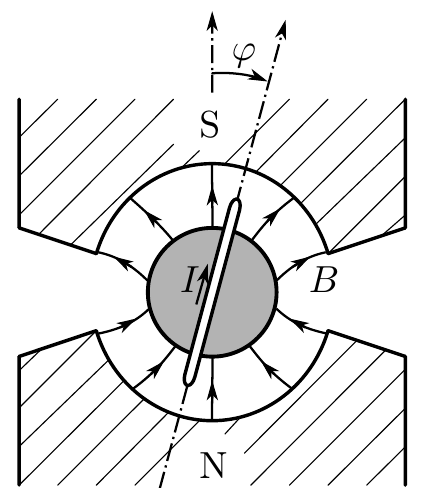
\includegraphics[width=6cm]{res/frame.png}
    	\label{fig:f}
    	\caption{Рамка с током в магнитном поле}
    \end{figure}
	
	
	Вращение рамки описывается уравнением моментов:
	
    \begin{equation}\label{main}
        \ddot{\varphi} + 2\gamma\dot{\varphi }+ \omega_0^2\varphi = K I,
    \end{equation}
    
    где $\varphi$ --- угол поворота рамки, $\gamma$ --- коэффициент затухания подвижной системы гальванометра, $\omega_0$ --- собственная частота колебаний рамки, $I = \frac{\varepsilon}{R_\Sigma}$ --- составляющая тока, вызванная внешней ЭДС, к которой подключён гальванометр, $K$ --- некоторый коэффициент.
    
    $\gamma$, $\omega_0$ и $K$ рассчитываются по следующим формулам:
        
    \begin{equation}
       K = \dfrac{BSN}{J}, \;\;\; 2\gamma \approx \dfrac{(BSN)^2}{JR_\Sigma}, \;\;\; \omega_0^2 = \dfrac{D}{J},
    \end{equation}
    
    где $B$ --- магнитное поле, в которое помещена рамка, $S$ --- площадь витка рамки, $N$ --- число витков рамки, $J$ --- момент инерции системы, $R_\Sigma$ --- сопротивление рамки и цепи, $D$ --- модуль кручения нити.


\subsection*{Режим измерения постоянного тока}

	Если через рамку пропускать постоянный ток (достаточно долго, чтобы затухли колебания подвижной системы), то в уравнении \eqref{main} можно положить $\ddot{\varphi} = 0, \; \dot{\varphi } = 0$, и угол поворота определится формулой
	
	\begin{equation}\label{C2}
	\varphi = \dfrac{K}{\omega_0^2}I = \dfrac{BSN}{D}I = S_I I = \dfrac{I}{C_1},
	\end{equation}
	
	где $C_I = \dfrac{1}{S_I}$ --- динамическая постоянная гальванометра.
	
\subsection*{Свободные колебания}
	
	При отсутствии внешнего источника тока, мы получаем следующее уравнение: 
	
	\begin{equation}\label{main}
    \ddot{\varphi} + 2\gamma\dot{\varphi }+ \omega_0^2\varphi = 0.
    \end{equation}
    
    В качестве начальных условий возьмём:

    \begin{equation}\label{B}
    \varphi(0) = 0,\; \dot{\varphi } = \dot{\varphi_0}.
    \end{equation}
    
    Рассмотрим возможные случаи движения рамки.
    
    \begin{enumerate}
    
        \item $\gamma < \omega_0$(колебательный режим).
    
            Решение уравнения (\ref{C2}) с начальными условиями (\ref{B}) имеет вид
            \begin{equation}
                \varphi \left( t \right) = \frac{\dot{\varphi_0}}{\omega_1} e^{-\gamma t} \sin{\omega_1 t},\;\;\; \omega_1 = \sqrt{\omega_0^2-\gamma^2}.
            \end{equation}
            
            Период колебаний в этом случае:
            
            \begin{equation}
                T_1 = \frac{2\pi}{\omega_1}=2\pi \left[\frac{D}{J}- \frac{\left( BSN \right)^4}{\left( 2 J R_Sigma \right)^2} \right]^{-1/2}
            \end{equation}
        
        \item $\gamma = \omega_0$(критический режим).
        
            Решение:
            \begin{equation}
                \varphi \left( t \right) = \dot{\varphi_0} t e^{-\gamma t}.
            \end{equation}
            
            Этот режим реализуется при сопротивлении внешнего участка цепи R, равном критическому сопротивлению:
            
            \begin{equation}
                R_\text{кр}=R_{\Sigma_\text{кр}}-R_0=\frac{(BSN)^2}{2\sqrt{D J}}-R_0.
            \end{equation}
            
        \item $\gamma > \omega_0$(затухание велико).
        
            Решение
            \begin{equation}
                \varphi (t) = \frac{\dot{\varphi_0}}{\alpha} e^{-\gamma t} \sh (\alpha t), \;\;\; \alpha = \sqrt{\gamma^2-\omega_0^2}.
            \end{equation}
            
    \end{enumerate}
    
\subsection*{Режим измерения заряда}
	
	Период свободных колебаний баллистического гальванометра благодаря искусственному увеличению момента инерции рамки оказывается очень большим (порядка десяти секунд). Если пропустить через рамку короткий импульс тока, то можно считать, что весь ток успевает пройти при неотклоненном положении рамки. Рамка, однако, при этом получает толчок, в результате которого возникает движение, описываемое уравнением свободных колебаний при начальных условиях $\varphi(t) = 0, \; \dot{\varphi }(0) = \dot{\varphi }_0$.

	Для вычисления скорости $ \dot{\varphi }_0 $, полученной в результате толчка, умножим уравнение \eqref{main} на $ dt $ и проинтегрируем его по времени от 0 до момента окончания токового импульса $ \tau $. Пренебрегая малыми вторым и третьим членом в левой части, получаем,
	
	\begin{equation}
	   \int\limits_0^\tau \ddot{\varphi}dt = K 	\int\limits_0^\tau I dt \Rightarrow \dot{\varphi }(\tau) = K_q
	\end{equation}
	
	где $q$ --- полный электрический заряд, прошедший через рамку за время импульса. При этом мы пренебрегаем зарядом индукционного тока.
	
	
	Величина $ C_Q = \dfrac{q}{\varphi_{max}}$ называется баллистической постоянной гальванометра. Баллистическая постоянная наряду с динамической является важнейшей характеристикой гальванометра, но в отличие от динамической она существенно зависит от режима работы гальванометра (от сопротивления цепи).
	
	Расчёт показывает, что максимальный отброс достигается при полном
	отсутствии затухания (тормозящий индукционный ток отсутствует при
	обрыве в цепи):
	
	\begin{equation}\label{}
	\varphi_{max}^\text{св} = \dfrac{\dot{\varphi }(\tau) }{\omega_0} = \dfrac{Kq}{\omega_0}
	\end{equation}
	
	В этом случае, однако, возникшие в результате отброса колебания рам-
	ки не будут успокаиваться, и прибор не скоро сможет быть использован
	для повторных измерений.
	
	Обычно удобнее всего работать в режиме, близком к критическому:
	
	\begin{equation}\label{bal2}
	\varphi_{max}^\text{кр} = \dfrac{Kq}{\omega_0 e} = \frac{\varphi_{max}^\text{св}}{e}
	\end{equation}
	
	Таким образом, в критическом режиме максимальное отклонение зайчика в $ e $ раз меньше, чем в режиме свободных колебаний. Отсюда, в частности,  следует, что отношение баллистических постоянных
	
	\begin{equation}\label{}
	\dfrac{C_{Q}^\text{кр}}{C_{Q}^\text{св}} = e.
	\end{equation}
	


	\section*{Экспериментальная установка}

	\subsection*{Стационарный ток}
	
	В режиме стационарного тока можно легко вычислить ток по формуле 
	
	\begin{equation}\label{I}
	I = \dfrac{R_1}{R_2} \dfrac{U_0}{R + R_0}
	\end{equation}
	
	Координата $ x $ зайчика связана с углом $ \varphi $ простым соотношением $ x = a\tg 2\varphi $. При малых $ \varphi  =  \dfrac{x}{2a}$, где $ a $ --- расстояние от шкалы до зеркальца. 
	
	Отсюда из \eqref{C2} получаем:
	
	\begin{equation}
	C_I = \frac{2 a I}{x} \; \Rightarrow \; I = \frac{C_I}{2a}x.
	\label{eq:din}
	\end{equation}
	
    Т. е. зависимость $I(x)$ линейная с коэффициентом наклона $k=\frac{C_I}{2a}$.
    
    \begin{figure}[h!]
    	\centering
    	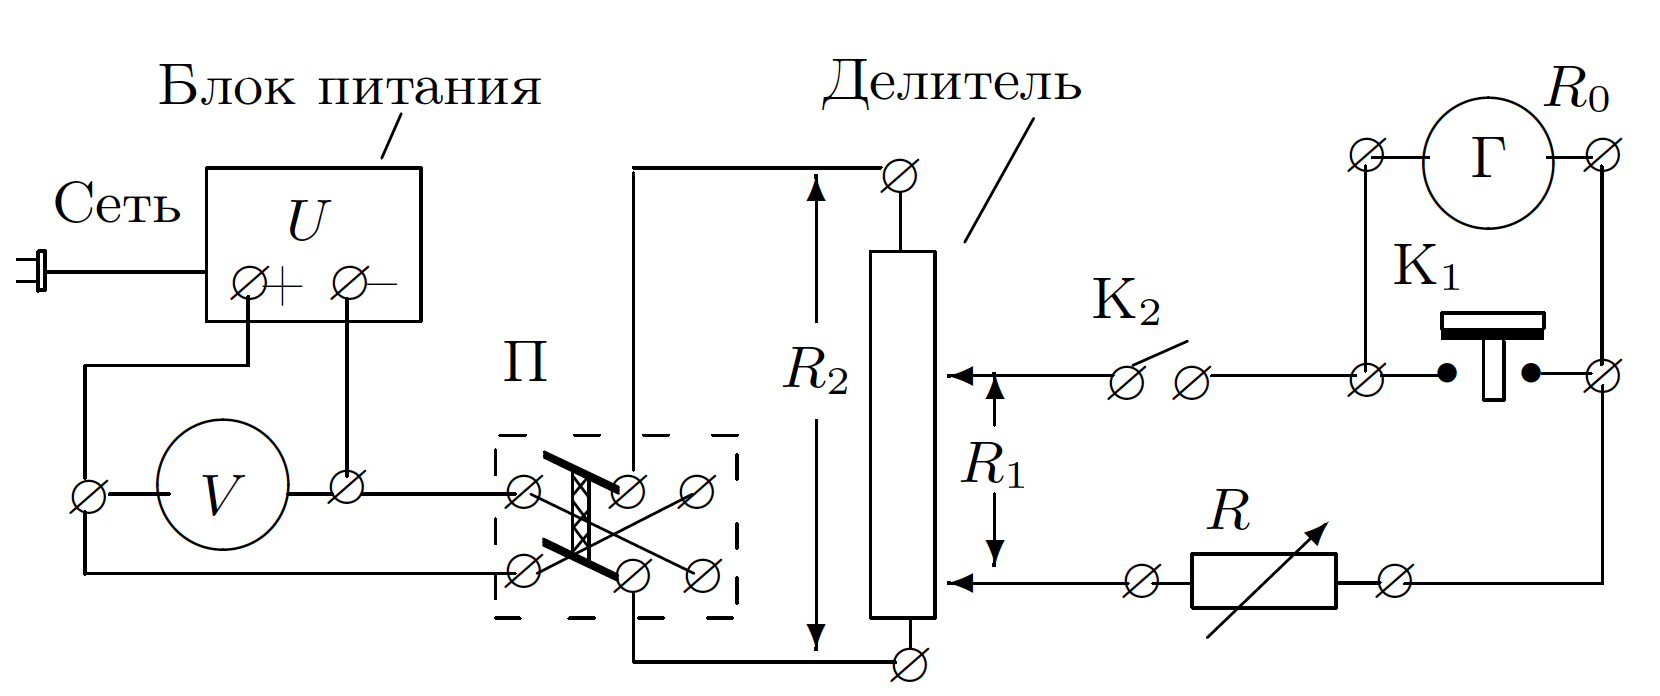
\includegraphics[width=10cm]{res/scheme1.png}
    	\caption{Схема установки для работы гальванометра в стационарном режиме}
    	\label{s1}
    \end{figure}

	
	\subsection*{Критический режим и свободные колебания}
	
	Логарифмический декремент затухания определяется экспериментально по формуле
	
	\begin{equation}\label{Theta}
	\Theta =  \gamma T =  \ln \dfrac{x_k}{x_{k+n}}
	\end{equation}
	
	При этом мы можем выразить декремент как
	
	\begin{equation}\label{}
		\Theta =  \gamma T =  \dfrac{2\pi\gamma}{\sqrt{\omega_0^2 - \gamma^2}} = \dfrac{2\pi R_3}{\sqrt{(R + R_0)^2 - R_3^2}}
	\end{equation}
	
	где $ R_3 = R_\text{кр} + R_0 $. Отсюда нетрудно получить формулу: 
	
	\begin{equation}\label{}
	\dfrac{4\pi^2}{\Theta^2} = \dfrac{(R_0 + R)^2}{(R_0 + R_\text{кр})^2} - 1
	\end{equation}
	
	Для расчета $ R_\text{кр} $, перепишем предыдущую формулу:
	
	\begin{equation}\label{Rkr}
	R + R_0 = (R_0 + R_\text{кр})\sqrt{\frac{4\pi^2}{\Theta^2} + 1}
	\end{equation}
	
	Т. е. зависимость $(R+R_0)\left(\sqrt{\frac{4\pi^2}{\Theta^2} + 1}\right)$ линейная с коэффициентом наклона $k$. Следовательно 
	
	\begin{equation}\label{Rkr}
	    R_\text{кр} = k - R_0.
	\end{equation}
	 
	 
	 \subsection*{Баллистический режим}
	 
    \begin{figure}[h!]
    	\centering
    	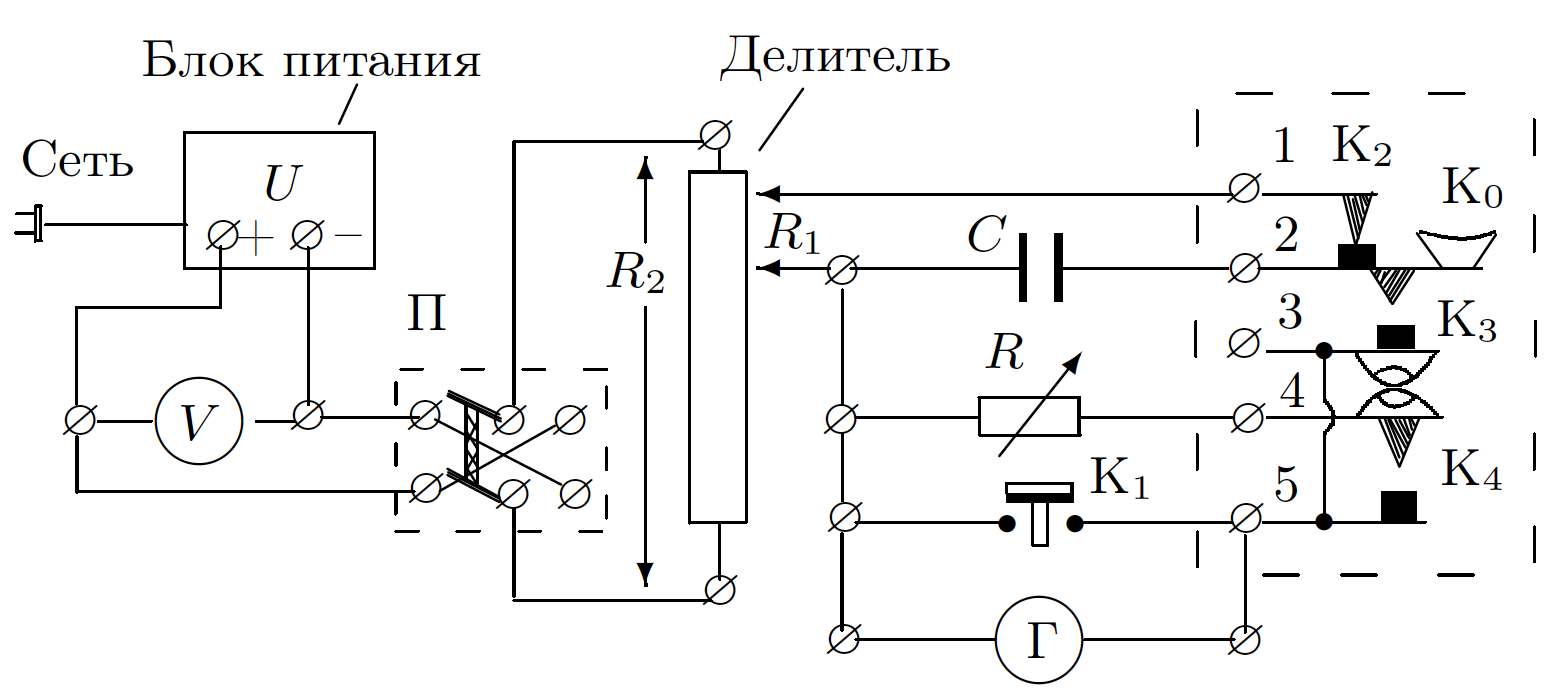
\includegraphics[width=10cm]{res/scheme2.png}
    	\label{fig:s2}
    	\caption{Схема установки для определения баллистической постоянной}
    \end{figure}

	 
	 Заряд конденсатора $ C $ равен 
	 
	 \begin{equation}\label{}
	    q = C U_C  = C U_0 \dfrac{R_1}{R_2}
	 \end{equation}
	 
	 Из решения уравнения колебаний и формулы декремента следует формула 
	 
	 \begin{equation}\label{eq:bal}
	 \varphi_{max}^\text{св} = \varphi_0 e^{\Theta_0/4} \approx \varphi_0 \left(1+\Theta_0/4\right)
	 \end{equation}
	 
	 При сопротивлении, равном критическому, баллистическая постоянная будет определяться
	 
	 \begin{equation}
	 C_{q}^\text{кр} = \dfrac{q}{\varphi_{max}^\text{кр}} = 2a\dfrac{R_1}{R_2}\dfrac{U_0C}{x_{max}^\text{кр}}
	 \label{C}
	 \end{equation}


\section*{Ход работы}

\subsection*{Определение динамической постоянной}

Соберем схему согласно рис. \ref{s1} и занесём её параметры в таблицу \ref{default}. Установим делитель на $\frac{R_1}{R_2} \approx \frac{1}{2000}$. Подберём сопротивление магазина $R_{max} = 8$ кОм, при котором зайичк отклонится на $l_{max} = 22.7$ см. 

\begin{table}[H]
	\caption{Характеристики установки}
	\begin{tabular}{ccccc}
\toprule
$S\cdot N, \text{см}^2\cdot\text{вит}$ & $r_\text{внеш}, \text{Ом}$ &  $a, \text{мм}$ &  $L_{3,5}, \text{мм}$ &  $l, \text{мм}$ \\
\midrule
72 & $<=5$ & 1,5 & 3,0 & 1,7 \\
\bottomrule
\end{tabular}
	\label{default}
\end{table}

Снимем зависимость отклонения зайчика $x$ от сопротивления магазина $R$ при $U_0=1.50$ В и рассчитаем соответсвующие токи. Результаты измерений занесём в таблицу \ref{table:din}. Построим также для наглядности графики $x(R)$ и, рассчитав по формуле \ref{I}, $I(x)$.

\begin{table}[H]
	\caption{Зависимость сопротивления магазина, отклонения зайчика и тока}
	\begin{tabular}{ccc}
\toprule
$R$, \text{кОм} & $x$, см &  $I$, $\text{мкА}$\\
\midrule
8  & 22.7 & 88.24 \\
10 & 18.5 & 71.43 \\
12 & 15.7 & 60.00 \\
14 & 13.7 & 51.72 \\
16 & 12.1 & 45.45 \\
18 & 10.8 & 40.54 \\
20 & 9.9  & 36.59 \\
30 & 6.9  & 24.59 \\
40 & 5.4  & 18.52 \\
50 & 4.5  & 14.85 \\
\bottomrule
\end{tabular}

		\label{table:din}
\end{table}

\begin{figure}[H]
	\caption{График зависимости отклонения зайчика от сопротивления магазина}
	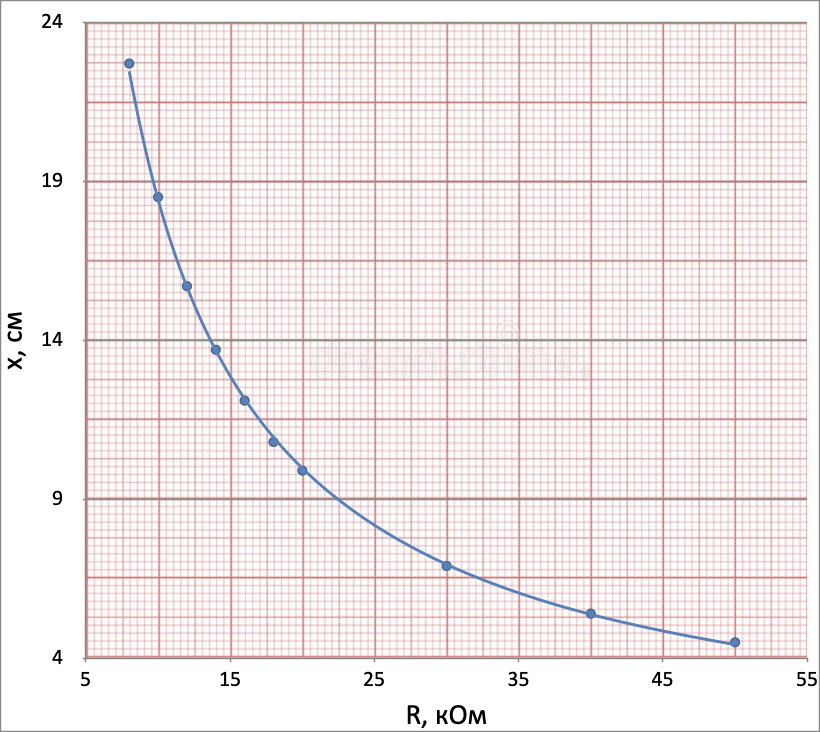
\includegraphics[width = 9.8 cm]{src/xR.png}
	\label{fig:plt1}
\end{figure}

\begin{figure}[H]
	\caption{График зависимости тока от отклонения зайчика}
	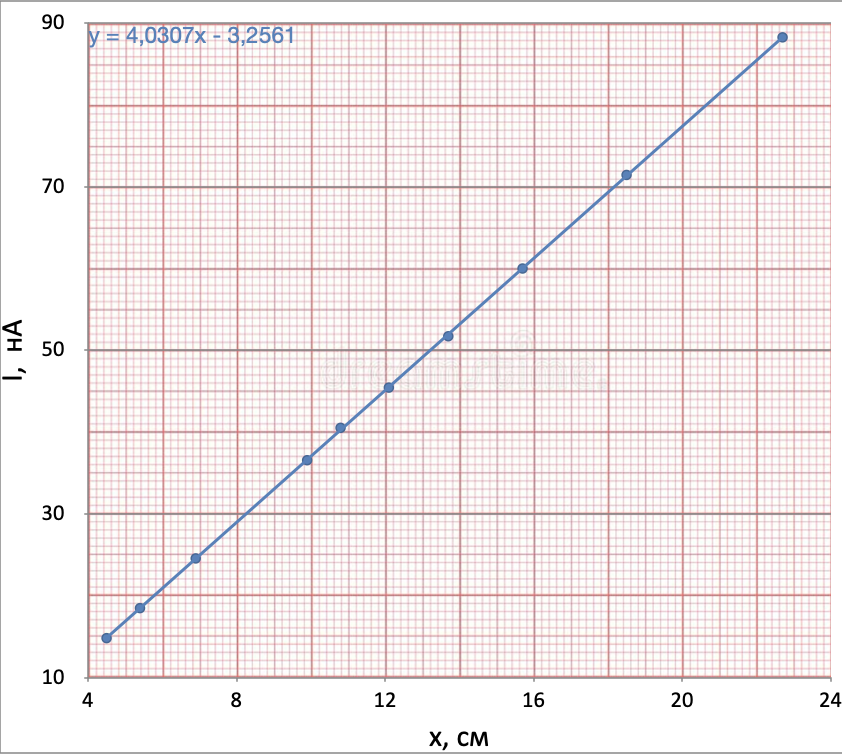
\includegraphics[width = 9.8 cm]{src/Ix.png}
	\label{fig:plt2}
\end{figure}

Параметры зависимости $I(x)$ занесем в таблицу \ref{table:mnk1}.

\begin{table}[H]
	\caption{Результаты обработки зависимости $I(x)$}
	\begin{tabular}{l|ccc}
	\toprule
	 & $k$, $\frac{\text{мА}}{\text{мм}/\text{м}}$ & $\varepsilon_k$, \% \\ \midrule
	$I=k\cdot{x}$ & 4.03 & 0.4 \\
\bottomrule
\end{tabular}
	\label{table:mnk1}
\end{table}

Тогда по формуле \ref{eq:din}: 
    $$ C_I = 0.97 \pm 0.006\; \frac{\text{мА}}{\text{мм}/\text{м}} \;\;\; \varepsilon_{C_I} = 0.6\%. $$



\subsection*{Определение критического сопротивление}

Для начала измерим период $T_0$ свободных колебания рамки при сопротивлении $R$ = 8 кОм. 
Период 7 колебаний --- 38.82 с. Значит $T_0=5.55$ с.

Также определим логарифмический коэффициент затухания $\Theta_0$ разомкнутого гальванометра, пользуясь формулой \ref{theta}. Данные занесём в таблицу \ref{theta}.

$$\Theta_0 = 0.218 \pm 0.003 \;\;\; \varepsilon_{\Theta_0} = 2\%$$

\begin{table}[H]
	\caption{Данные для определения коэффициента затухания}
	\begin{tabular}{cc}
\toprule
$x_n$, \text{см} & $\ln\left(\frac{x_n}{x_{n+1}}\right)$ \\
\midrule
17.9 & 0.225 \\
14.3 & 0.218 \\
11.5 & 0.223 \\
9.2  & 0.218 \\
7.4  & 0.210 \\
6.0  & 0.203 \\
4.9  & 0.228 \\
3.9  &       \\ 
\bottomrule
\end{tabular}

		\label{theta}
\end{table}

Далее определим критическое сопротивление. Для этого подберем наибольшее сопротивление магазина, при котором при размыкании ключа $\text{П}$ зайчик не переходит за нулевое значение. Получаем  $R_\text{кр} \approx 8.3 \pm 0.1$ кОм. 

Теперь для расчёта $ \Theta $  проведём измерение отклонений зайчика после размыкания ключа $ \text{П} $, увеличивая $ R $ магазина от $ 3R_\text{кр} $  до $ 10R_\text{кр} $. Подсчитаем при этом логарифмический декремент по формуле \eqref{Theta}. Результаты занесём в таблицу \ref{thetaR}. Построим график зависимости $(R+R_0)\left(\sqrt{\frac{4\pi^2}{\Theta^2} + 1}\right)$ и найдём $R_\text{кр}$ по формуле \ref{Rkr}.

\begin{table}[H]
	\caption{Результаты измерений и расчётов для определения $R_\text{кр}$}
	\begin{tabular}{cccccc}
\toprule
$R$, \text{кОм} & $x_n$, см & $x_{n+1}$, см & $\Theta$ &  $\sqrt{\frac{4\pi^2}{\Theta^2} + 1}$ & $R+R_0$, кОм\\
\midrule
25 & 14.3 & 2.0 & 1.97 & 3.35 & 25.5 \\
29 & 12.1 & 2.1 & 1.75 & 3.72 & 29.5 \\
33 & 10.8 & 2.3 & 1.55 & 4.18 & 33.5 \\
37 & 9.8  & 2.4 & 1.41 & 4.58 & 37.5 \\
41 & 9.1  & 2.5 & 1.29 & 4.96 & 41.5 \\
46 & 7.9  & 2.5 & 1.15 & 5.55 & 46.5 \\
50 & 7.4  & 2.6 & 1.05 & 6.09 & 50.5 \\
57 & 5.7  & 2.2 & 0.95 & 6.68 & 57.5 \\
83 & 4.7  & 2.4 & 0.67 & 9.40 & 83.5 \\
\bottomrule
\end{tabular}

		\label{thetaR}
\end{table}

\begin{figure}[H]
	\caption{График зависимости $(R+R_0)\left(\sqrt{\frac{4\pi^2}{\Theta^2} + 1}\right)$}
	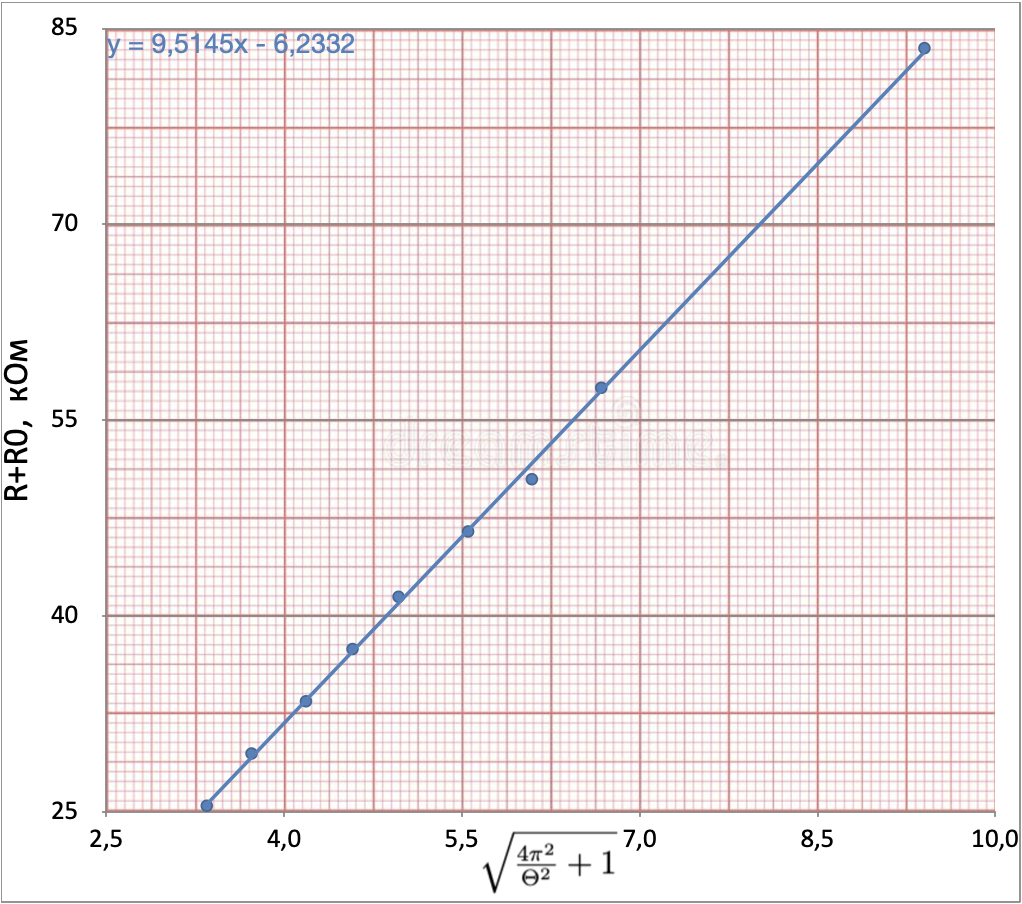
\includegraphics[width = 9.5 cm]{src/Rkrit.png}
	\label{fig:plt2}
\end{figure}

\begin{table}[H]
	\caption{Результаты обработки зависимости $(R+R_0)\left(\sqrt{\frac{4\pi^2}{\Theta^2} + 1}\right)$}
	\begin{tabular}{l|ccc}
	\toprule
	 & $k$, $\text{кОм}$ & $\varepsilon_k$, \% \\ \midrule
	$R+R_0=k \cdot \sqrt{\frac{4\pi^2}{\Theta^2} + 1}$ & 9.51 & 2 \\
\bottomrule
\end{tabular}
	\label{table:mnk1}
\end{table}

Тогда по формуле \ref{eq:din}: 
    $$ R_\text{кр} = 9.01 \pm 0.2\; \text{кОм} \;\;\; \varepsilon_{R_\text{кр}} = 2\%. $$


\subsection*{Баллистический режим}

Выставим на делителе $\frac{R_1}{R_2} = \frac{1}{70}$, т. к. при таком отношении $\frac{R_1}{R_2}$ первый отброс $x_0$ = 22.2 см, что составляет практически всю шкалу. Тогда по формуле \ref{eq:bal}:
$$x_{max}^\text{св} = 22.2 \cdot e^{0.218/4} = 23.4 \;\;\; \text{см}.$$
По формуле  \ref{bal2}: $$x_{max}^\text{кр}=\frac{23.4}{2.7}=8.6 \;\;\; \text{см}.$$

Снимем зависимость первого отброса $x_{max}\left(R+R_0\right)$. Результаты измерений и обработки занесём в таблицу \ref{tab:bal}. Для нахождения $R_\text{кр}$ построим график $x_{max}\left(R+R_0\right)$. 
Проинтерполируем график функцией $x_{max}=4.7321 \ln(R+R_0)-0.1223$. Тогда:
$$R_\text{кр}=e^{\frac{x_{max}^\text{кр}+0.1223}{4.7321}}-R_0=5.82 \;\;\; \text{кОм}$$

Найдём $C_q^\text{кр}$ по формуле \ref{C}:
$$C_q^\text{кр} = 1.2 \pm 0.02\; \frac{\text{мКл}}{\text{мм}/\text{м}} \;\;\; \varepsilon_{C_q}= 1.7\%$$
А также время релаксации:
$$\tau = R_0 C = 1 \; \text{мс} \; \ll \; T_0 = 5.55 \; \text{с}.$$


\begin{table}[H]
	\caption{Результаты измерений и обработки в баллистическом режиме}
	\begin{tabular}{ccc}
\toprule
$x$, см & $R$, кОм &  $R+R_0$, кОм\\
\midrule
18.5 & 50 & 50.50 \\
17.3 & 40 & 40.50 \\
16.5 & 30 & 30.50 \\
14.4 & 20 & 20.50 \\
11.1 & 10 & 10.50 \\
9.5  & 8  & 8.50  \\
8.3  & 6  & 6.50  \\
6.6  & 4  & 4.50  \\
4.0  & 2  & 2.50  \\
2.6  & 1  & 1.50  \\
\bottomrule
\end{tabular}
	\label{tab:bal}
\end{table}

\begin{figure}[H]
	\caption{График зависимости $x_{max}\left(R+R_0\right)$}
	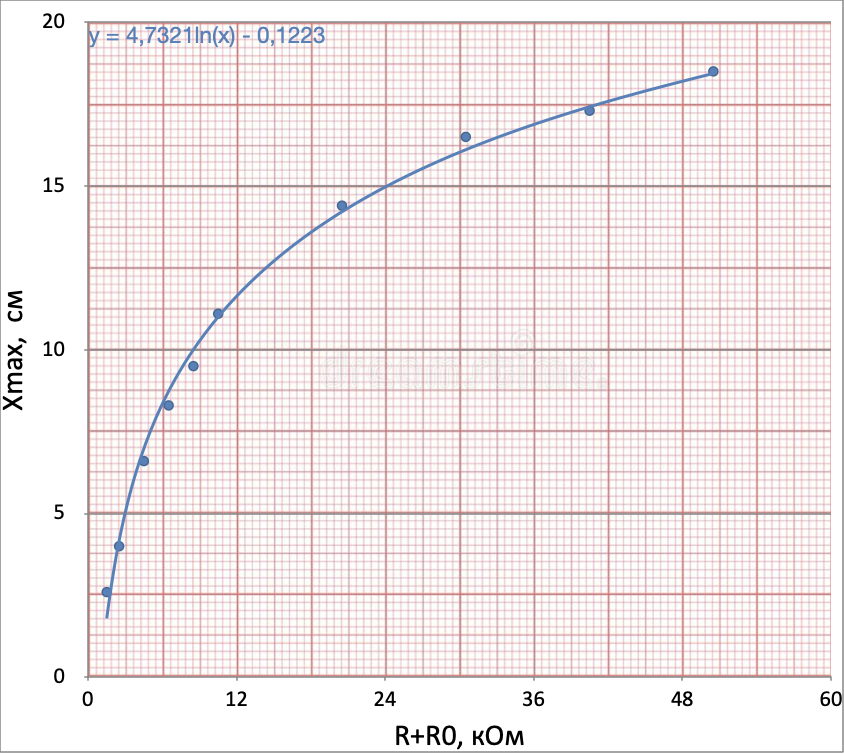
\includegraphics[width = 9.8 cm]{src/xRR0.png}
	\label{fig:plt2}
\end{figure}

\section*{Вывод}

В ходе работы были получены следующие значения для параметров установки:
$$C_I = 0.97 \pm 0.006\; \frac{\text{мА}}{\text{мм}/\text{м}} \;\;\; \varepsilon_{C_I} = 0.6\%. $$
$$C_q^\text{кр} = 1.2 \pm 0.02\; \frac{\text{мКл}}{\text{мм}/\text{м}} \;\;\; \varepsilon_{C_q}= 1.7\%$$
Был определён период свободных колебаний:
$$T_0=5.55 \; \text{с}$$
Логарифмический коэффициент затухания:
$$\Theta_0 = 0.218 \pm 0.003 \;\;\; \varepsilon_{\Theta_0} = 2\%$$
Было определено критическое сопротивление тремя способами:\newline

С помощью подбора:  $R_\text{кр} \approx 8.3 \pm 0.1$ кОм;\newline

С помощью линеаризации зависимости $R(\Theta)$: $$ R_\text{кр} = 9.01 \pm 0.2\; \text{кОм} \;\;\; \varepsilon_{R_\text{кр}} = 2\%. $$ 
С помощью зависимости $x_{max}(R)$: $R_\text{кр} = 5.82$ кОм.

\newpage
\begin{thebibliography}{9}
	\bibitem{Siv} Сивухин Д. В. \emph{Общий курс физики. Том 3 Электричество и магнетизм}, 2004
	\bibitem{kirich} Кириченко Н.А. \emph{Электричество и магнетизм.}, 2011
	\bibitem{max} \emph{Лабораторный практикум по общей физике. В 3 томах. Том 2. Электричество и магнетизм: учебное пособие} под ред. А. В. Максимычева, М. Г. Никулина
\end{thebibliography}

\end{document}
